% !TeX root = ../main.tex
\chapter{架构}\label{ch5}

多年来,深度学习领域已经为每个应用领域开发了多种深度架构,这些架构在多个人们关注的标准方面表现出良好的折中:例如 训练便捷性、预测准确性、内存占用、计算成本、可扩展性等。

\section{多层感知机}\label{sec5.1}

最简单的深度架构是\keyterm{多层感知机}(\keyterm{MLP}),它由一系列\keyterm{全连接层}组成,层与层之间通过\keyterm{激活函数}分隔。请参见图 \ref{fig5.1} 中的示例。由于历史原因,在这样的模型中,\keyterm{隐藏层}的数量指的是线性层的数量,不包括最后一层。

\begin{figure}
    \centering
    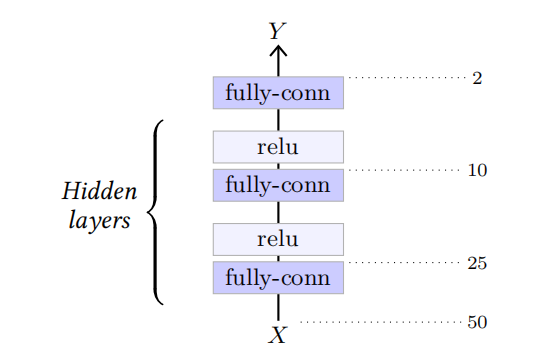
\includegraphics[width=0.9\textwidth]{fig/fig5.1.png}
    \caption[多层感知机]{该多层感知器以大小为 $50$ 的一维张量作为输入,由三个全连接层组成,输出维度分别为 $25$、$10$ 和 $2$,前两个层后面是 ReLU 层。}
    \label{fig5.1}
\end{figure}

一个关键的理论成果是\keyterm{通用逼近定理} \citep{Cybenko1989},该定理指出,如果激活函数 $\sigma$ 是连续的且非多项式的,那么任意连续函数 $f$ 都可以在紧致域上被形式为 $l_2 \circ \sigma \circ l_1$ 的模型任意精确地一致逼近,其中紧致域是有界的并包含其边界,$l_1$ 和 $l_2$ 是仿射的。这样的模型是一个只有单个隐藏层的多层感知机(\keyterm{MLP}),这个结果意味着它可以近似任何具有实用价值的东西。然而,这种逼近成立的条件是第一个线性层的输出维度可以任意大。

尽管 MLP 很简单,但当要处理的信号维度不太大时,它仍然是一个重要的工具。

\section{卷积网络}\label{sec5.2}

处理图像的标准架构是\keyterm{卷积网络},也称 \keyterm{convnet},它结合了多个\keyterm{卷积层},既可以在信号被\keyterm{全连接层}处理之前降低信号大小,也可以输出一个同样较大尺寸的二维信号。

\subsubsection*{类 LeNet}

用于图像\keyterm{分类}的原始 \keyterm{LeNet} \citep{Lecun98} 模型结合了一系列充当特征提取器角色的二维\keyterm{卷积层}和\keyterm{最大池化}层,以及一系列充当 \keyterm{MLP} 并实际执行分类任务的\keyterm{全连接层}(见图 \ref{fig5.2})。

\begin{figure}
    \centering
    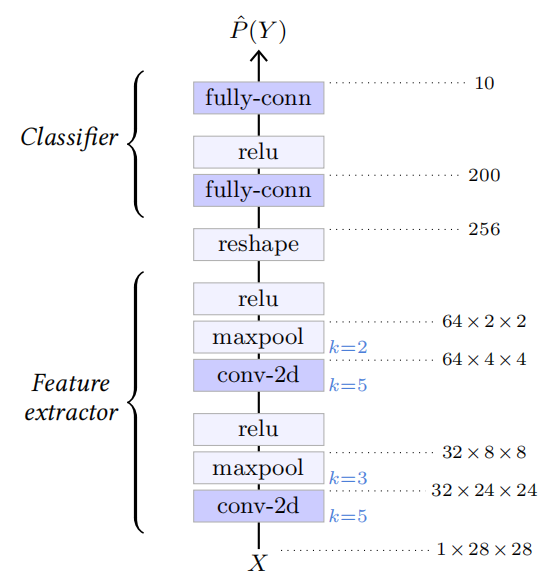
\includegraphics[width=0.9\textwidth]{fig/fig5.2.png}
    \caption[类 LeNet 卷积模型]{用于对手写数字的 $28 \times 28$ 灰度图像进行分类的小型 \keyterm{LeNet} 网络示例 \citep{Lecun98}。它的前半部分是卷积层,交替使用卷积层和最大池化层,将信号维度从 $28 \times 28$ 个标量减少到 $256$。它的后半部分通过一个隐藏层感知器处理这个 $256$ 维特征向量,以计算 $10$ 个 logit 分数对应十个可能的数字。}
    \label{fig5.2}
\end{figure}

这一架构为许多具有相同结构的模型提供了蓝图,这些模型只是在规模上更大大,例如 AlexNet \citep{nips-1502.c399862d3b9d6b76c8436e924a68c45b} 或 VGG系列 \citep{arxiv-1409.1556}。

\subsubsection*{残差网络}

遵循 LeNet 家族架构的标准卷积神经网络不易于扩展为深层架构,并且会遇到梯度消失问题。\citep{arxiv-1512.03385} 提出的 \keyterm{残差网络}(ResNets)明确解决了梯度消失问题,它们通过\keyterm{残差连接}(详见 \ref{sec4.7} 节),使得网络能够拥有数百层。残差网络已成为计算机视觉应用的标准架构,并且根据层数的不同存在多个版本。我们将详细探讨用于分类的 \keyterm{ResNet-50} 架构。

\begin{figure}
    \centering
    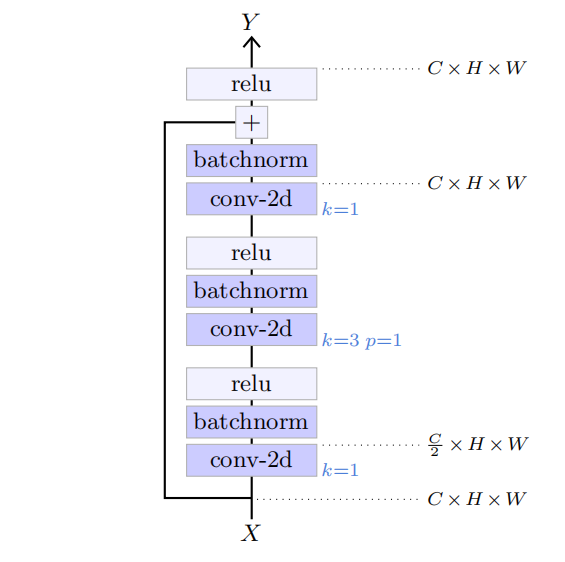
\includegraphics[width=0.9\textwidth]{fig/fig5.3.png}
    \caption[残差块]{残差块}
    \label{fig5.3}
\end{figure}

与其他 ResNet 一样,ResNet-50 由一系列\keyterm{残差块}组成,每个残差块结合了多个\keyterm{卷积层}、\keyterm{批归一化}层和 ReLU 层,并包裹在残差连接中。如图 \ref{fig5.3} 所示。

在处理真实图像时,要实现高性能的一个关键要求是传递具有大量通道的信号,以允许丰富的表征。然而,卷积层的参数数量及其计算成本与通道数呈二次方关系。这种残差块通过首先使用 $1 \times 1$ 卷积减少通道数来缓解这一问题,然后在减少的通道数上用 $3 \times 3$ 卷积进行空间操作,之后再次通过 $1 \times 1$ 卷积放大通道数。

\begin{figure}
    \centering
    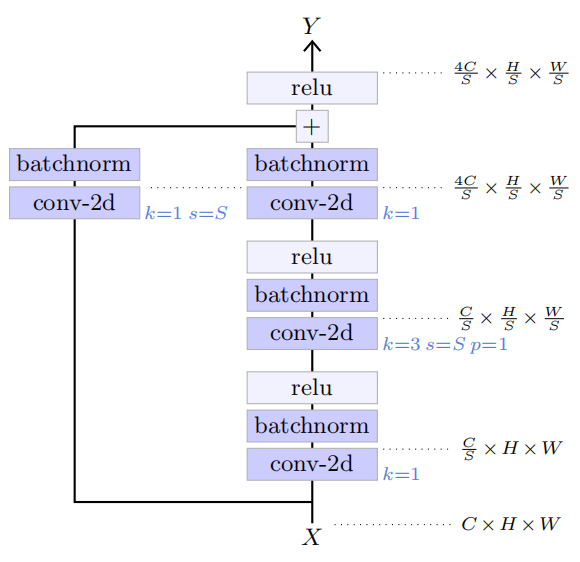
\includegraphics[width=0.9\textwidth]{fig/fig5.4.png}
    \caption[下采样残差块]{下采样残差块接受一个元参数 $S$,即第一个卷积层的步长,用于调节张量尺寸的缩减程度。}
    \label{fig5.4}
\end{figure}

该网络通过减少信号的维度来最终计算用于分类的 logit 值。这得益于一个由几部分组成的架构,每个部分都以一个\keyterm{下采样残差块}开始,其将信号的高度和宽度减半,并将通道数加倍,然后是一系列残差块。这样的下采样残差块具有与标准残差块相似的结构,不同之处在于它需要一个改变张量形状的残差连接。这是通过步长为 $2$ 的 $1 \times 1$ 卷积实现的(参见图 \ref{fig5.4})。

\begin{figure}
    \centering
    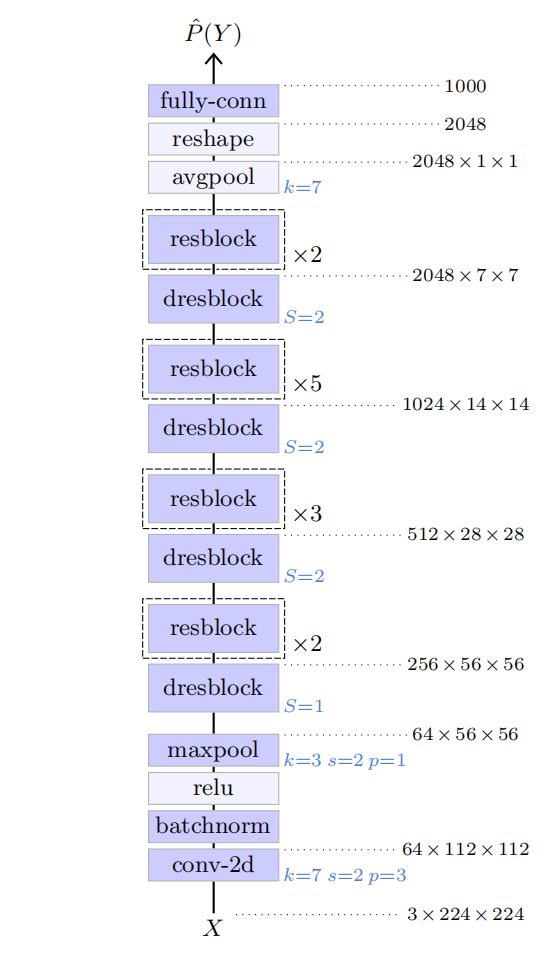
\includegraphics[width=0.9\textwidth]{fig/fig5.5.png}
    \caption[ResNet-50]{ResNet-50 的结构 \citep{arxiv-1512.03385}}
    \label{fig5.5}
\end{figure}

ResNet-50 的整体结构如图 \ref{fig5.5} 所示。 它从 $7 \times 7$ 卷积层开始,将三通道输入图像转换为尺寸减半的 $64$ 通道图像,随后是四部分残差块。令人惊讶的是,在第一部分中,并没有下采样,只是将通道数增加了 $4$ 倍。最后一个残差块的输出是 $2048 \times 7 \times 7$,其通过一个 $7 \times 7$ 核大小的平均池化被转换为 $2048$ 维的向量,然后通过全连接层处理以获得最终的 logit 值,此处为 $1000$ 个类别。

\section{注意力模型}\label{sec5.3}

\subsubsection*{Transformer}

\subsubsection*{生成式预训练 Transformer}

\subsubsection*{视觉 Transformer}